\documentclass[11pt]{article}
\usepackage[review]{acl}
\usepackage{amsmath,amssymb,amsthm}
\usepackage{booktabs,multirow,array,tabularx,graphicx,xcolor,url,listings,enumitem,microtype,tikz}
\usetikzlibrary{arrows.meta,positioning,fit,backgrounds}
\definecolor{codegray}{gray}{0.95}
\lstset{basicstyle=\ttfamily\footnotesize,backgroundcolor=\color{codegray},frame=single,framesep=3pt,framerule=0.4pt,xleftmargin=3.4pt,xrightmargin=3.4pt,breaklines=true,columns=fullflexible,keepspaces=true,showstringspaces=false,tabsize=2}
\newtheorem{theorem}{Theorem}
\newtheorem{proposition}{Proposition}
\newtheorem{definition}{Definition}
\newtheorem{assumption}{Assumption}
\title{Truthprint: Typed Invariant Contracts for Translation-Robust Authenticated Semantic Provenance}
\author{Anonymous ACL Submission}

\begin{document}
\maketitle

\begin{abstract}
Token-level LLM watermarks are fragile under translation and paraphrasing because their signal lives in surface tokens. We propose \emph{Truthprint}, a semantic intermediate representation that separates \emph{locked invariants} (polarity, quantity, time, attribution, roles) from \emph{controlled realization} via a machine-checkable typed mutability contract. What survives transformation is \emph{ledger-based authenticated semantic provenance}---a keyed tag over the invariant digest, re-verified after transformation---not an in-text watermark: hiding a payload in realization freedom is a negative result under real MT (a surface parser recovers $0/192$ NLLB outputs). On $4{,}800$ real NLLB translations across six languages, a Stage-2 extractor recovers the invariants ($0.83$--$0.99$) and the scheme attributes translated documents cross-lingually (core6 document attribution $0.90$--$1.000$), rejecting single-field tampers ($\ge0.996$) and \emph{localizing} the changed field---unlike a token watermark (KGW), a SemStamp-style embedding-region detector (at matched FPR), or robust hashing. Rule-based benign paraphrase is authenticated ($1.00$); a fixed-lexicon adaptive attacker removes the mark, but open-vocabulary neural frontends defend even held-out attacks (ValidRemoval $0.05$--$0.10$). We prove three \emph{conditional} properties reducing to the MAC and show that the operative false-positive floor is the contract-collision rate, not $2^{-\tau}$. All results are closed-domain and small-scale; Truthprint verifies consistency with a participating keyed generator, not arbitrary AI text.
\end{abstract}

\paragraph{Keywords.} Intermediate representation, authenticated provenance, LLM watermarking, semantic provenance, translation robustness

\section{Introduction}
Large language models can generate fluent text at scale, creating a growing need for provenance mechanisms that survive ordinary content transformation. Generation-time watermarking modifies the decoding process so that an authorized detector can identify a statistical signature in generated text. SynthID-Text demonstrated that such watermarking can be integrated into sampling without retraining the underlying LLM and can be detected without rerunning the generator \cite{dathathri2024synthid}.

Regulation motivates machine-readable marking under Article~50 of the EU AI Act \cite{euaiact2024}, useful only if robust \cite{liu2024survey}; we treat robustness as a technical objective, not a compliance claim. Provenance also aids data hygiene, since training on unattributed synthetic text degrades models over generations \cite{shumailov2024collapse}.

Token-level methods, however, embed their signal in surface token choices. Translation, paraphrasing, sentence restructuring, and summarization replace many of those choices while preserving substantial meaning. This creates a structural mismatch: the desired provenance claim concerns the persistence of content identity, whereas the carrier often depends on language-specific lexical decisions.

Recent semantic watermarks use sentence embeddings, contextual representations, or structured graphs \cite{hou2024semstamp,ren2024semmark,liu2023sir,ye2026swan,schaefer2026dew}, but semantic similarity alone does not distinguish meaning that must never change from choices that may safely vary: two sentences can be embedding-close yet differ in negation, quantity, temporal scope, attribution, modality, or causal direction.

This paper proposes \emph{Truthprint}, a typed semantic IR for provenance that explicitly separates:
\begin{enumerate}[leftmargin=*]
  \item \textbf{semantic invariants}, which must remain fixed; and
  \item \textbf{controlled realization variables}, which may encode watermark symbols only when semantic and pragmatic equivalence is validated.
\end{enumerate}

The central novelty is a machine-checkable contract that fixes which semantic fields are locked and which realization choices may vary; it both constrains an in-text watermark and, as a keyed tag over the locked fields, authenticates meaning out of band. Figure~\ref{fig:pipeline} shows the end-to-end data flow.

The delta over the closest prior work is precise. Embedding-based semantic watermarks \cite{hou2024semstamp,ren2024semmark,liu2023sir,schaefer2026dew} define admissibility through a \emph{metric} (closeness under a learned distance); Truthprint defines it through a \emph{typed predicate}---admissible only when a symbolic invariant relation holds field by field---so a watermark symbol ranges over key-dependent invariant-equivalence classes rather than tokens or embedding regions (Sec.~\ref{sec:analysis}). Conditional on sound extraction, encoding stays within a class and preserves protected fields, and because attribution is gated by a payload bound to the invariant digest, fresh-payload forgery reduces to MAC security. SWAN \cite{ye2026swan} shares a graph carrier but adopts an existing formalism wholesale, whereas Truthprint types each field with an explicit mutability policy validated before release.

\subsection{Contributions}
\begin{itemize}[leftmargin=*]
  \item \textbf{Method.} We formulate watermark carriers as secret-keyed realization choices constrained by a field-level mutability contract (\emph{locked}/\emph{conditional}/\emph{realization-only}), combining uncertain-carrier erasures, error correction, and invariant-bound payload authentication.
  \item \textbf{Conditional analysis.} Assuming sound invariant extraction and validation we establish protected-field fidelity; under standard cryptographic assumptions fresh-payload forgery and per-test tag acceptance reduce to the MAC; and we show the operative false-positive floor is the contract-collision rate, with a measured crossover to the $2^{-\tau}$ bound.
  \item \textbf{Reproducible real-MT evidence.} On $4{,}800$ committed NLLB translations across six languages the meaning layer survives and authenticates cross-lingually where surface carriers and a real token watermark do not; at a matched FPR it beats a SemStamp-style embedding-region detector and robust hashing and alone rejects \emph{and} localizes single-field tampers; it stays specific when the verifier must search the ledger without a document id; and open-vocabulary neural frontends defend held-out adaptive attacks. All Truthprint numbers reproduce from committed data with no GPU; wide-coverage parsing and scale remain open.
\end{itemize}

\paragraph{Claim--evidence boundary.} Table~\ref{tab:claims} (appendix) separates what the artifact \emph{demonstrates}, what is proved only under explicit assumptions, and what remains a hypothesis (e.g., ``language-neutral'' names the intended schema interface, not a measured property).

\begin{figure*}[t]
\centering
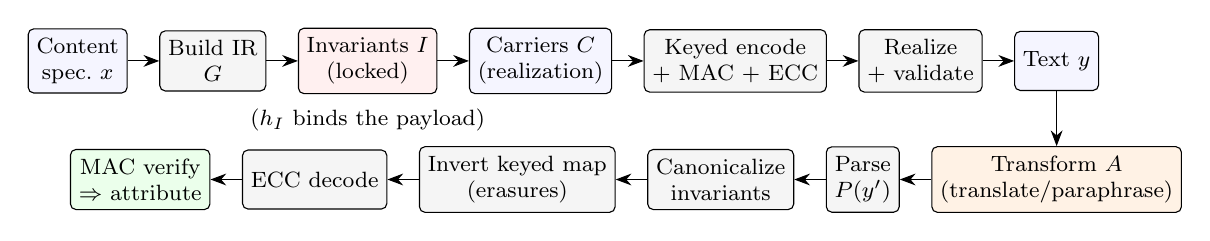
\begin{tikzpicture}[
  font=\footnotesize,
  box/.style={draw, rounded corners=2pt, align=center, minimum height=7.5mm,
              inner xsep=3pt, fill=blue!4},
  lock/.style={draw, rounded corners=2pt, align=center, minimum height=7.5mm,
               inner xsep=3pt, fill=red!6},
  op/.style={draw, rounded corners=2pt, align=center, minimum height=7.5mm,
             inner xsep=3pt, fill=black!4},
  >={Stealth[length=2mm]}
]
\node[box] (x) {Content\\spec.\ $x$};
\node[op, right=4mm of x] (build) {Build IR\\$G$};
\node[lock, right=4mm of build] (inv) {Invariants $I$\\(locked)};
\node[box, right=4mm of inv] (car) {Carriers $C$\\(realization)};
\node[op, right=4mm of car] (enc) {Keyed encode\\$+$ MAC $+$ ECC};
\node[op, right=4mm of enc] (real) {Realize\\+ validate};
\node[box, right=4mm of real] (y) {Text $y$};
\draw[->] (x)--(build); \draw[->] (build)--(inv); \draw[->] (inv)--(car);
\draw[->] (car)--(enc); \draw[->] (enc)--(real); \draw[->] (real)--(y);

\node[op, below=7mm of y, fill=orange!10] (att) {Transform $A$\\(translate/paraphrase)};
\draw[->] (y)--(att);

\node[op, left=4mm of att] (parse) {Parse\\$P(y')$};
\node[op, left=4mm of parse] (canon) {Canonicalize\\invariants};
\node[op, left=4mm of canon] (invert) {Invert keyed map\\(erasures)};
\node[op, left=4mm of invert] (ecc) {ECC decode};
\node[box, left=4mm of ecc, fill=green!8] (verify) {MAC verify\\$\Rightarrow$ attribute};
\draw[->] (att)--(parse); \draw[->] (parse)--(canon); \draw[->] (canon)--(invert);
\draw[->] (invert)--(ecc); \draw[->] (ecc)--(verify);

\node[below=1.5mm of inv, font=\footnotesize, inner sep=1pt] {($h_I$ binds the payload)};
\end{tikzpicture}
\caption{Truthprint data flow. Encoding (top, left$\to$right) locks the
invariant set $I$, maps an authenticated, error-corrected payload onto
realization carriers $C$, and validates every candidate against the contract
before emitting text. Detection (bottom, right$\to$left) re-parses possibly
transformed text, canonicalizes invariants, inverts the keyed map with
erasures, decodes, and attributes only on MAC verification. The invariant
digest $h_I$ binds the payload, so an invariant-altering transform breaks
attribution (Proposition~\ref{thm:fpr}). Under real MT the in-text carrier path is
a negative result (Sec.~\ref{sec:realmt}); the mechanism that survives is the
out-of-band ledger tag over $h_I$, re-verified after re-extraction
(Sec.~\ref{sec:provenance}).}
\label{fig:pipeline}
\end{figure*}

\section{Background and Related Work}
\paragraph{Token-level and provable watermarks.}
The green--red list watermark \cite{kirchenbauer2023kgw} and SynthID-Text \cite{dathathri2024synthid,synthidgithub,hf_synthid}, which generalizes it via tournament sampling, embed a keyed statistic in token selection; analysis shows detector robustness depends on its statistical assumptions \cite{omidi2026synthidanalysis}. A parallel line seeks formal guarantees: provable robustness for a unigram watermark \cite{zhao2023provable}, distortion-free editing-robust watermarks \cite{kuditipudi2024distortionfree}, cryptographically undetectable watermarks \cite{christ2024undetectable}, publicly verifiable unforgeable watermarks \cite{liu2024unforgeable}, and low-FPR statistical tests \cite{fernandez2023threebricks}. All carry the signal in token decisions, which meaning-preserving transformations replace; He et al.\ show token watermarks lack cross-lingual consistency and are removed by pivot translation \cite{he2024crosslingual}. Truthprint inherits the cryptographic spirit at the \emph{provenance} layer---fresh-payload unforgeability and per-candidate tag acceptance (Propositions~\ref{thm:unforge},~\ref{thm:fpr}) reduce to MAC security---with no claim of undetectability.

\paragraph{Semantic and structured watermarks.}
Embedding-region and semantic-context methods---SemStamp \cite{hou2024semstamp}, SemaMark \cite{ren2024semmark}, semantic-invariant watermarking \cite{liu2023sir}, dual embeddings \cite{schaefer2026dew}---reduce token dependence; SWAN carries the signal in AMR structure \cite{ye2026swan}, and SynGuard hybridizes token masking with semantic alignment \cite{han2025synguard}. But embedding geometry does not expose \emph{which} typed fact changed: high similarity can coexist with altered polarity, quantity, attribution, modality, or causal direction. Truthprint instead defines a watermark-specific typed IR, assigns each field a mutability policy, and validates every realization against an immutable contract before release.

\paragraph{Attacks and robust hashing.}
\label{sec:relhash}
Watermark presence and family can be identified by black-box probing \cite{gloaguen2024blackbox}, motivating a Kerckhoffs threat model (security in the key, not obscurity); scrubbing and spoofing under distillation \cite{yi2025unifiedattacks} and radioactive traces in fine-tuned models \cite{sander2024radioactive} motivate MAC-authenticated payloads rather than statistical agreement; and detector-guided adversarial paraphrasing \cite{cheng2025adversarial} motivates counting a removal as successful only when it both evades detection and preserves meaning:
\begin{multline}
\label{eq:validremoval}
\mathrm{ValidRemoval}=\mathbf{1}\big[D_K(y')<\tau_D\big]\\
\cdot\,\mathbf{1}\big[\mathrm{InvariantEq}(P(y),P(y'))=1\big].
\end{multline}
Registering a meaning-digest tag and re-verifying it after transformation resembles \emph{robust hashing} (MinHash \cite{broder1997minhash}, SimHash \cite{charikar2002simhash}, learned semantic hashing), but those answer a \emph{similarity} question that cannot localize a typed field change---a single-field edit stays within tolerance (Sec.~\ref{sec:matched}). Truthprint instead hashes a \emph{typed invariant contract} with a keyed MAC, a typed, keyed member of that family whose false-positive floor is the analyzed contract-collision probability (Sec.~\ref{sec:provenance}). Table~\ref{tab:positioning} (appendix) positions it against representative systems.

\section{Problem Definition}
For a content specification $x$, secret key $K$, payload $m$, encoder $E_K$, language-$\ell$ realizer $R_\ell$, transformation $A$, multilingual parser $P$, and detector $D_K$, the generated text is $y=R_\ell(E_K(x,m))$, an observed transform is $y'=A(y)$, and detection returns $(s,\hat{m},c)=D_K(P(y'))$ (score, recovered payload or prefix, confidence report). The design targets four objectives: (i)~\emph{semantic fidelity} $I(P(y))=I(x)$ for invariant extractor $I$; (ii)~\emph{natural-language quality} above deployment thresholds (not evaluated here); (iii)~\emph{robust detection} under transformations that preserve sufficient invariant and carrier evidence; and (iv)~\emph{controlled authenticated false positives}---under the stated PRF and independence assumptions an independently produced decoded payload rarely passes the keyed tag check, with the statistical fallback separately calibrated.

\section{Threat Model}
\paragraph{Benign transformations.} The detector should tolerate Unicode normalization, punctuation changes, spelling correction, translation, round-trip translation, synonym substitution, active--passive alternation, clause splitting and merging, sentence-level paraphrasing, moderate paragraph rewriting, and limited insertion or deletion; this paper evaluates translation, round-trip translation, and sentence-level paraphrase.

\paragraph{Attackers.} A non-adaptive attacker applies off-the-shelf translation, paraphrasing, or summarization without knowing $K$. An adaptive attacker may know the schema and detector design, repeatedly rewrite text, splice documents, target known carrier families, or query an exposed detector.

\paragraph{Out of scope.} Truthprint does not identify all AI-generated text. It verifies consistency with a participating keyed generator. Absence of a signal does not prove human authorship.

\section{Truthprint Intermediate Representation}
\subsection{Three-Layer Structure}
A Truthprint document contains three conceptual layers.

\textbf{Layer A: Semantic invariants.} Entities, predicates, semantic roles, polarity, negation scope, modality, quantities, temporal intervals, causal direction, conditions, exceptions, attribution, quotation status, and uncertainty.

\textbf{Layer B: Controlled realization variables.} Voice, event/state framing, clause packaging, discourse-connective family, proposition ordering, nominal/verbal realization, anaphoric choice, and optional explanatory apposition.

\textbf{Layer C: Provenance and coding metadata.} Scheme identifier, key identifier, payload, nonce, error-correcting-code parameters, carrier assignments, reliability estimates, invariant digest, and optional signed server-side provenance.

\subsection{Typed Mutability}
Each field $f$ is assigned $\mathrm{Mutability}(f)\in\{\mathrm{locked},\mathrm{conditional},\mathrm{realization\mbox{-}only}\}$: locked fields never change, conditional fields change only when context-specific validators approve, and realization-only fields may carry watermark symbols.

\subsection{Example Representation}
A simplified representation (locked predicate/roles/polarity/time with a realization space over voice and event framing) is given in Appendix~\ref{app:pseudocode}.
\section{Formal Semantic Contract}
A Truthprint graph is $G=(V_E,V_V,E_R,E_D,\Phi)$---entity nodes, event/state nodes, semantic-role edges, discourse/logical relations, and scoped features such as negation, modality, time, quantity, and attribution---partitioned as $G=I\cup C\cup U$ into the invariant set $I$, the controlled carrier set $C$, and unconstrained style $U$. A transformed structure $G'$ is admissible only when $\mathrm{InvariantEq}(I(G),I(G'))=1$ and $Q(R_\ell(G'))\ge\tau_Q$ for a quality and contextual-consistency function $Q$. Hard invariants are validated symbolically where possible; soft invariants such as emphasis or pragmatic implication require bidirectional entailment, contradiction checks, and human-calibrated thresholds.

\section{Watermark Encoding}
\label{sec:validation}
The raw payload may carry a generator-family, deployment, coarse time-bucket, nonce, and policy identifier---never personal identifiers, prompts, or exact timestamps. The authenticated payload is $p=m\parallel\mathrm{MAC}_K(m\parallel n\parallel h_I)$ for nonce $n$ and canonical invariant digest $h_I$, error-corrected as $c=\mathrm{ECC}(p)$ following prior robust multi-bit watermarking \cite{qu2024multibitecc}. The encoder discovers admissible carrier families per discourse unit (voice, clause packaging, discourse-connective family, nominal/verbal realization, proposition order), rejecting context-inappropriate ones such as a passive that obscures an important agent. For carrier $j$ with alternatives $A_j=\{a_{j,0},\ldots,a_{j,r-1}\}$, a keyed permutation $\pi_j=\mathrm{PRP}_K(\mathrm{CanonicalHash}(I,G,j,n))$ selects $a_j^\star=\pi_j(c_j\bmod|A_j|)$; because the map depends on the invariant graph and nonce, no global rule such as ``passive means 1'' exists. Each realized candidate is reparsed and checked for hard-invariant equality, bidirectional entailment, numerical and entity consistency, fluency, and expected carrier recoverability; if none is valid the carrier is recorded as an erasure rather than forcing degraded text. Encoding and detection pseudocode are in Appendix~\ref{app:pseudocode}.



\section{Watermark Detection}
\label{sec:detection}
Detection segments the document, identifies language, parses each segment into Truthprint, resolves entities, normalizes predicates and roles, canonicalizes quantities and time, and extracts observable carrier alternatives. For an observed carrier $a_j^{obs}$ it reconstructs the keyed permutation and derives $\hat{c}_j=\pi_j^{-1}(a_j^{obs})$, treating uncertain observations as erasures; an ECC decoder reconstructs candidate payloads, accepted only when their MAC verifies. When complete recovery is impossible, a calibrated fallback over $n$ reliable binary carriers with $k$ keyed matches uses
\begin{equation}
z=\frac{k-0.5n}{\sqrt{0.25n}},
\label{eq:zscore}
\end{equation}
whose production calibration must account for dependence among carrier observations.



\section{Formal Analysis}
\label{sec:analysis}
We state what the design guarantees given sound primitives; what depends on semantic parsing is measured empirically (Sec.~\ref{sec:experiments}), and computational complexity is in Appendix~\ref{app:complexity}.

\subsection{Carriers as Invariant-Equivalence Classes}
\begin{definition}[Invariant equivalence]
Let $I(\cdot)$ be the invariant extractor. Two structures $G,G'$ are invariant-equivalent, written $G\sim_I G'$, iff $\mathrm{InvariantEq}(I(G),I(G'))=1$. For a discourse unit with invariants $I$, the admissible realization set is
\begin{equation}
\mathcal{R}(I)=\{\,r : I(P(r))=I \ \land\ Q(r)\ge \tau_Q\,\}.
\end{equation}
\end{definition}
A carrier alphabet $A_j$ is a key-dependent partition of $\mathcal{R}(I)$ into classes; the encoder selects a class by symbol and the realizer emits any member. Thus the watermark ranges over the quotient $\mathcal{R}(I)/{\sim_I}$ rather than over tokens or embedding neighborhoods.

\begin{assumption}[Validator soundness]
\label{as:validator}
The hard-invariant validator $V$ is sound: if $V$ accepts a candidate $r$ for invariants $I$, then $I(P(r))=I$. (It need not be complete; rejected admissible candidates only reduce capacity, not fidelity.)
\end{assumption}

\begin{proposition}[Conditional protected-field fidelity]
\label{prop:fidelity}
Under Assumption~\ref{as:validator}, every committed output $y=R_\ell(E_K(x,m))$ satisfies $I(P(y))=I(x)$.
\end{proposition}
\begin{proof}[Proof sketch]
Encoding commits a candidate only if $V$ accepts it, and carriers with no accepted candidate are recorded as erasures rather than realized (Sec.~\ref{sec:validation}). By soundness, acceptance implies invariant equality for that unit; taking the conjunction over committed units gives $I(P(y))=I(x)$.
\end{proof}
Logit-biasing methods lack such an in-loop invariant check, so they can only measure quality preservation post hoc.

\paragraph{Empirical validator soundness.}
We measure the load-bearing assumption as the validator's false-accept rate on single-field tampers. On the closed domain the typed contract flags every tamper across all six fields (property C1, $1.000$, CI $[0.998,1.000]$) while retaining attribution across benign paraphrase ($0.990$); a decode-only ablation accepts every tamper (C2, $0.000$), confirming that invariant re-extraction---not the coding layer---supplies soundness. Under real NLLB translation the Stage-2 extractor still rejects meaning-altering edits at $\ge0.99$ per condition (Sec.~\ref{sec:provenance}). Wide-coverage validator soundness remains open, so Proposition~\ref{prop:fidelity} stays conditional.

\subsection{Unforgeability and False Positives}
\begin{proposition}[Fresh-payload unforgeability; standard reduction]
\label{thm:unforge}
Model the tag as $t=\mathrm{MAC}_K(m\parallel n\parallel h_I)$ truncated to $\tau$ bits. Any PPT adversary that causes authenticated attribution for a tuple $(m,n,h_I)$ not previously tagged by the generator yields an EUF-CMA forgery against this truncated MAC with the same success probability (up to simulation overhead). Thus its success is bounded by the EUF-CMA advantage of the instantiated truncated MAC; guessing loss is already part of that advantage and is not added a second time.
\end{proposition}
\begin{proof}[Proof sketch]
Attribution requires a recovered payload whose tag equals $\mathrm{MAC}_K(m\parallel n\parallel h_I)$ on a triple not produced by the generator. The reduction answers authorized generation requests with its tagging oracle and, when the detector accepts a fresh tuple, outputs that tuple and recovered tag as its forgery. Replay of a previously tagged tuple is excluded by freshness and must instead be handled by deployment policy.
\end{proof}

\begin{proposition}[Authenticated acceptance under an ideal-PRF model]
\label{thm:fpr}
Assume the truncated MAC is a pseudorandom function on a fresh input and the decoded candidate tag is independent of its output. For a fixed (key, nonce) test, an independently produced candidate payload passes the $\tau$-bit tag check with probability $2^{-\tau}$, up to the PRF distinguishing advantage. For $Q$ tested key--nonce pairs, the union bound is $Q2^{-\tau}$ plus that advantage.
\end{proposition}
This bounds only a candidate that reaches tag verification: for $q$ fresh candidates whose tags are independent of ideal-PRF outputs the union bound is $q2^{-\tau}$ ($2.3\times10^{-10}$ at $\tau{=}32$), \emph{not} an end-to-end detector FPR---parsing, candidate search, replay, carrier dependence, and threshold calibration all affect system-level error, and replayed outputs require a nonce registry. The $0/20000$ observation of Sec.~\ref{sec:impl} is consistent with the bound (approx.\ $95\%$ binomial upper bound $1.5\times10^{-4}$). When full recovery fails, the fallback $z$ of Eq.~\eqref{eq:zscore} satisfies $\Pr[z\ge t\mid H_0]\le e^{-t^2/2}$ under independent binary carriers, calibrated in deployment.

Carrier capacity and the minimum reliable text length for the in-text channel are analyzed in Appendix~\ref{app:capacity}.

\section{Experiments}
\label{sec:experiments}
\paragraph{Setup.} All data are \emph{synthetic template facts} in one closed domain (software incidents: four agents, four patients, one predicate---\emph{fix}, with \emph{break} used only as a tamper value---and two to four closed values each for polarity, quantity, time direction, modality, attribution, and causation, so core6 has $192$ possible values); the main corpus is $50$ documents $\times16$ sentences, translated by NLLB-200-distilled-600M into Korean, Hindi, Chinese, Arabic, and German and round-trip into English ($4{,}800$ outputs). The \emph{Stage-1} frontend parses surface carriers; the \emph{Stage-2} frontend is a hand-built six-language lexicon that extracts the nine invariant fields. A \emph{contract} is the field subset that is authenticated: core6 (polarity, quantity, time, attribution, predicate, agent) or full9 (all nine). Because the extractor and the corpus share one closed vocabulary, these results establish feasibility, not open-domain accuracy. Runs are seeded; rates carry Wilson $95\%$ CIs; implementation, protocol, and hypotheses are in the appendix.

\subsection{Surface carriers: a negative result under real MT}
\label{sec:realmt}
Translating $4$ documents of $16$ templated sentences with a real system (NLLB-200-distilled-600M) into Korean/Hindi and back ($192$ outputs) and re-parsing each with the Stage-1 \emph{surface} frontend recovers $0/192$ (parse coverage $0.000$, CI $[0.000,0.020]$), including round-trip English. Hiding a payload in realization freedom therefore does not survive real translation; the bottleneck is wide-coverage parsing, not the coding or cryptographic core (Appendix~\ref{sec:impl}). Measuring carrier survival from the transformed text itself is essential---an annotation that merely \emph{asserts} survival reports a spurious perfect score.

\subsection{The meaning layer survives real translation (Stage-2)}
\label{sec:stage2}
A closed-domain lexicon extractor over six languages (English, Korean, Hindi, Chinese, Arabic, German) recovers the nine invariant fields from $4{,}800$ real NLLB translations ($800$ source sentences over $50$ documents $\times$ six conditions). Aggregate recovery (Wilson $95\%$ CI) is $0.83$--$0.99$: the small closed categoricals (polarity, quantity, attribution, time) survive at $\ge0.97$, while the open entity and relational fields are lower ($0.83$--$0.92$; patient $0.825$ weakest). Strict all-nine-field recovery is highest for Hindi/German ($0.69$/$0.66$) and lowest for Arabic ($0.25$), where MT renders entities most variably. Because the recovered fields fix the invariant digest, a meaning-altering edit to any field is detected across languages---direct real-data evidence that the meaning layer survives MT where the surface carriers of Sec.~\ref{sec:realmt} do not; a wide-coverage neural parser is the next step (\texttt{scripts/\allowbreak eval\_multilingual.py}).

\subsection{A wide-coverage neural frontend on open-domain text}
\label{sec:neural}
A feasibility pilot ($16$ base sentences, $6$ with open wording, in six conditions; $96$ records) ran an instruction LLM as a drop-in extractor: on \emph{closed} templates the hand-built lexicon leads ($0.970$ vs.\ $0.726$ field recovery), but on the open wording the lexicon degrades below the neural frontend ($0.481$ vs.\ $0.614$), strongest on typed relational fields (predicate $0.896$, causation $0.948$). Neural extraction is not yet reliable: it recovers all nine fields of a sentence in none of the $96$ records (lexicon $0.479$). The harness enforces \emph{separate} translation and extraction models (removing the self-consistency confound); a translator-independent embedding frontend (\texttt{model2vec}) recovers open-domain temporal direction at $0.944$ where the lexicon abstains, though a static embedding is insufficient for the full contract.

\subsection{Meaning-based provenance authentication under real translation}
\label{sec:provenance}
The producer registers a keyed $\tau$-bit tag ($\tau{=}32$) over the canonical digest of a declared \emph{invariant contract} (a field subset) in the out-of-band ledger; the verifier re-extracts the invariants (Stage-2) and authenticates iff the tag reproduces. On the $4{,}800$ translations a compact contract (polarity, quantity, time, attribution, predicate, agent) gives document-level attribution---a document attributed when $\ge$ half its sentences authenticate---of $1.000$ (CI $[0.929,1.000]$) for German and Hindi, $0.980$ round-trip, $0.940$ Korean/Chinese, and $0.900\,[0.786,0.957]$ Arabic over $50$ documents; sentence-level TPR $0.618$--$0.886$, tamper rejection $\ge0.996$, false positives $0.000$--$0.007$. Widening to nine fields raises meaning coverage but lowers TPR (AR $0.253$) and collapses attribution for the hardest conditions (AR $0.02$, ZH $0.08$, RT $0.24$) while German/Hindi hold at $0.94$---an explicit fidelity/robustness trade-off, and the translation-robust counterpart of the $0/192$ surface pilot. One caveat is quantitative: because authentication reproduces a tag over a \emph{contract}, two distinct low-entropy generations sharing a contract digest collide before the tag is tested, so the achievable false-positive floor is the \emph{contract-collision} probability set by the contract's entropy, not $\tau$. For the six-field contract this floor is $5.2\times10^{-3}$ ($\approx1/192$), matching the measured $0.000$--$0.007$ and $\sim\!2\times10^{7}\times$ the $2^{-32}$ bound; nine fields lower it to $\sim\!1.8\times10^{-4}$, and the $2^{-\tau}$ bound binds only once the entity-vocabulary entropy exceeds $\tau$ bits (Appendix~\ref{sec:impl}). These rates are \emph{id-addressed}: the verifier is told which registered sentence to test. Without an id (translation strips any in-text identifier) the verifier must search the ledger, and sentence-level search is not specific---a core6 sentence collides with some wrong entry of the $800$-sentence ledger in $0.66$--$0.87$ of cases. The ${\ge}50\%$ document rule restores specificity: searching all $50$ registered documents with no id, core6 attributes translated documents to their source at $0.90$--$1.00$ with $0/2{,}450$ false document attributions per condition ($95\%$ upper bound $1.6\times10^{-3}$ per document pair). Per-pair risk multiplies with ledger size; an independence model at the core6 floor predicts $\approx1.1\times10^{-5}$ per pair on this corpus, so ledgers beyond ${\sim}10^4$ documents need a higher-entropy contract (full9: $\approx5\times10^{-17}$). The NLLB run is committed (\texttt{paper/results/realmt\_b2/}); every number here reproduces with no GPU (\texttt{scripts/eval\_provenance.py}, \texttt{eval\_ledger\_search.py}).

\subsection{Baseline comparison: token, semantic, and robust-hashing}
\label{sec:baselines}\label{sec:matched}
A KGW token watermark with $\gamma{=}0.25,\delta{=}2.0$ \cite{kirchenbauer2023kgw} on GPT-2 generations, translated by the same NLLB system, loses document-level detection from $0.960$ clean to $0.000$--$0.380$ across six conditions, confirming cross-lingual token-watermark removal \cite{he2024crosslingual}; meaning-digest document attribution on our corpus stays at $0.90$--$1.00$ (Appendix Table~\ref{tab:baselines}). The two share the translator but not the source text, so this shows signal removal, not a controlled head-to-head. The controlled comparison scores every method at a \emph{matched} $1\%$ FPR on the same $800$ NLLB source sentences and their translations ($300$ bootstrapped $16$-sentence documents per condition; static multilingual embedding \texttt{model2vec}; Table~\ref{tab:matched}). The typed meaning-digest identifies every translated document in all six conditions ($1.000$); a SemStamp-style LSH detector \cite{hou2024semstamp}---our re-implementation, granted ideal generation---reaches $0.010$--$0.423$, embedding SimHash \cite{charikar2002simhash} $0.050$--$0.973$, and MinHash \cite{broder1997minhash} and SHA-256 nothing beyond the round trip. Template sentences lie close together in embedding space, which handicaps embedding methods: on a separate $16$-sentence LLM-MT set the SemStamp-style detector reaches $0.377$--$1.000$ (Appendix Table~\ref{tab:matched16}). In addition, a single-field meaning-altering edit is rejected by the typed contract ($1.000$, CI $[0.981,1.000]$) but by \emph{neither} similarity hash ($0.000$)---a near-duplicate fingerprint cannot see which typed field changed---while the exact hash that rejects every tamper also rejects every legitimate translation (Table~\ref{tab:matched}).


\begin{table}[t]
\centering
\caption{Matched-FPR comparison on the 800-sentence NLLB corpus: fraction of
translated $16$-sentence documents identified at a common $1\%$ FPR ($300$
bootstrapped documents per condition, seeded; static multilingual embedding).
RT $=$ round trip via Korean; KO/HI/ZH/AR/DE $=$ direct translation. Typed $=$ typed meaning digest; SemStamp is
our SemStamp-style LSH re-implementation with ideal generation; SimHash/MinHash
are robust hashes; SHA-256 is an exact hash. Only the typed contract both
survives translation and rejects a single-field tamper ($1.000$ vs.\ $0.000$ for
similarity hashes; in text).}
\label{tab:matched}
\footnotesize
\setlength{\tabcolsep}{3pt}
\begin{tabular*}{\linewidth}{@{}l@{\extracolsep{\fill}}cccccc@{}}
\toprule
Method & RT & KO & HI & ZH & AR & DE \\
\midrule
Typed          & 1.000 & 1.000 & 1.000 & 1.000 & 1.000 & 1.000 \\
SemStamp       & 0.423 & 0.027 & 0.077 & 0.040 & 0.010 & 0.020 \\
SimHash        & 0.973 & 0.587 & 0.560 & 0.767 & 0.050 & 0.500 \\
MinHash        & 0.753 & 0.000 & 0.000 & 0.000 & 0.000 & 0.000 \\
SHA-256        & 0.020 & 0.000 & 0.000 & 0.000 & 0.000 & 0.000 \\
\bottomrule
\end{tabular*}
\end{table}

\subsection{Ledger retrieval and NLI baselines}
\label{sec:retrieval}
Because the scheme already uses an out-of-band ledger, the natural control is to store the source and \emph{retrieve} it after transformation (bag-of-words cosine nearest neighbor), optionally with an NLI check. Under the same ledger and id-addressed verification, at benign acceptance of $0.94$/$0.92$ (typed digest $1.000$), plain retrieval and a directional-coverage NLI proxy reject essentially no single-field tamper ($0.047$/$0.061$; $0.139$/$0.151$ with a real multilingual encoder): a one-field edit stays nearest its own source. Only a \emph{perfect}, unrealizable oracle NLI matches the typed contract's $1.000$ rejection, and even then neither localizes the changed field nor yields a keyed tag, both of which the typed digest provides with no learned model in this closed domain (Appendix Table~\ref{tab:retrieval}).

\subsection{Paraphrase and adaptive-attack robustness}
\label{sec:paraphrase}
Rule-based, in-lexicon paraphrase (voice, time reflow, verb/time synonyms, hedge) authenticates at TPR $1.000$ and document attribution $1.000$, and a single-field altering edit is rejected at $1.000$. A schema-aware adaptive attacker that swaps the predicate verb and time expression for \emph{out-of-lexicon} synonyms achieves ValidRemoval (Eq.~\eqref{eq:validremoval}) $1.000$ under the \emph{closed} lexicon---a negative result we localize to exactly the abstained fields (predicate and time in all cases; attribution when present), with polarity and agent recovered in $100\%$ of attacks. The vulnerability is the fixed lexicon, not the meaning-digest: an \emph{extended-coverage} frontend drives it $1.000\!\to\!0.000$ at unchanged benign and tamper rejection, but a \emph{held-out} out-of-inventory attack still evades any fixed lexicon ($1.000$). The general defense is open-vocabulary parsing: two real instruction LLMs (schema-guided \texttt{neural\_parser}) drive the held-out novel ValidRemoval to $0.050$ (GPT-4o-mini, $N{=}40$) and $0.100$ (Llama-3.3-70B, $N{=}10$), both disjoint from the lexicons' upper CIs, at benign and tamper rejection $1.000$ (Appendix Tables~\ref{tab:neuraldefense},~\ref{tab:paraphrase}).

\section{Conclusion}
Truthprint is a typed semantic IR with a language-neutral schema interface for authenticated provenance whose key contribution is a machine-checkable separation between immutable meaning and controlled realization choices. What survives transformation is ledger-based authenticated semantic provenance---a keyed tag over the invariant contract, re-verified after translation or paraphrase---complementary to, not a replacement for, token-level watermarks. It cannot guarantee detection after arbitrary rewriting, but targets a narrower, defensible objective---preserving provenance across transformations that retain substantial meaning---which the real-MT evidence supports; wide-coverage parsing, official baselines, and scale remain future work.

\section*{Limitations}
Multilingual semantic parsing remains imperfect. Not every proposition admits multiple safe realization alternatives. Highly constrained text has low carrier capacity. Some apparently stylistic alternations change emphasis or information structure. Translation can omit modality, evidentiality, subjects, or discourse relations. Strong summarization can destroy both content and watermark evidence. Finally, candidate generation and semantic validation add computational overhead compared with direct token-level methods. The closed-domain adaptive paraphrase of Section~\ref{sec:paraphrase} shows the sharpest limitation directly: a schema-aware attacker who swaps out-of-lexicon content synonyms fully removes the meaning-digest under the closed lexicon while preserving meaning. An extended-coverage frontend defends that specific attack (ValidRemoval $1.000\!\to\!0.000$ without weakening tamper rejection); a held-out out-of-inventory attack still evades any fixed lexicon, but two real open-vocabulary neural runs (GPT-4o-mini $N{=}40$, Llama-3.3-70B $N{=}10$; Table~\ref{tab:neuraldefense}) defend even the held-out attack ($0.050$/$0.100$), establishing that wide-coverage \emph{open-vocabulary} parsing---not a longer lexicon---is the general defense. Those runs are closed-domain and modest in scale; the current artifact still does not evaluate real generators, human judgments, all official baselines, replay defenses, or open-vocabulary adaptive attacks \emph{at larger scale and across domains}. All evaluation data are synthetic template facts in one closed domain, read by a hand-built extractor that shares the corpus vocabulary; the matched-FPR comparison uses our own SemStamp-style re-implementation over a static embedding on template sentences that handicap embedding methods; the KGW comparison uses a GPT-2 generator on different source text; and id-free ledger attribution was measured only against a $50$-document ledger. Consequently it supports feasibility and closed-domain robustness claims, not comparative robustness or deployment readiness at wide coverage.

\section*{Ethical Considerations}
A provenance detector can be misused to accuse authors, censor content, or make automated disciplinary decisions. Truthprint therefore treats a positive result as evidence about a participating keyed generation system, not proof of AI authorship or of misconduct. Deployments should expose the tested scheme and key identifier, use independently calibrated error rates, preserve an appeal path, and avoid adverse decisions based on the detector alone. Absence of a mark is likewise not evidence of human authorship.

The design has dual-use risks: public carrier families can aid removal attacks, while secret or overly detailed payloads can enable tracking. Payloads should exclude personal identifiers, prompts, and precise timestamps; keys and nonce registries require access control, rotation, and audit. Evaluation text should be licensed or consented, human annotation should be compensated and documented, and language-specific error disparities should be reported rather than hidden in an aggregate score. The present artifact uses synthetic template facts, no personal data, and no human subjects; the real-MT pilot (Secs.~\ref{sec:realmt}--\ref{sec:provenance}) translates those synthetic facts with a public open-weights model (NLLB-200-distilled-600M) and involves no personal data or human subjects. Any scaled evaluation that adds human invariant or factual-equivalence annotation must use licensed or consented text and compensated, documented annotation.

\bibliography{references}
\appendix

\section{Reference Implementation and Verification}
\label{sec:impl}
To make the guarantees above concrete and reproducible, we provide a self-contained reference implementation (\texttt{reference/truthprint\_poc.py}, standard library only) of the language-independent core: the canonical invariant digest $h_I$, the authenticated payload $p=m\parallel\mathrm{MAC}_K(\cdot)$, the invariant-bound keyed carrier map, and a systematic GF(2) code with erasure decoding. This deliberately excludes the semantic parser so that the cryptographic and coding properties can be validated in isolation from model-dependent NLP. It exercises four properties and reports the following verified behavior (message $\mu=16$ bits, tag $\tau=32$ bits, code $[N,k]=[96,48]$):
\begin{itemize}[leftmargin=*]
  \item \textbf{P1 (round-trip recovery).} An invariant-preserving transform that re-realizes carriers and erases $28/96$ sites still yields exact payload recovery and a verifying MAC.
  \item \textbf{P2 (invariant binding).} Flipping a locked field (polarity positive$\to$negative) changes $h_I$, so the MAC fails and the document is \emph{not} attributed, illustrating Proposition~\ref{prop:fidelity}'s contract.
  \item \textbf{P3 (cryptographic false positives).} Over $20{,}000$ independent documents, $0$ were attributed. This is consistent with Proposition~\ref{thm:fpr}; statistically, the observation alone only gives an approximate 95\% binomial upper bound of $1.5\times10^{-4}$.
  \item \textbf{P4 (no global rule).} For a fixed symbol, $43/96\approx N/2$ realized options differ between two documents whose invariants differ, confirming the map is bound to $(K,h_I,n)$.
\end{itemize}
Table~\ref{tab:erasure} reports decode success versus carrier erasure rate for
the implemented $[96,48]$ code and seeded random-erasure protocol: full
recovery ($\geq0.998$) through $\epsilon=0.42$, followed by $0.982$ at
$\epsilon=0.44$, $0.774$ at $\epsilon=0.48$, $0.290$ at $\epsilon=0.50$, and
zero observed recovery at $\epsilon\geq0.52$. The location and shape are
finite-code measurements; only the necessary survivor-count boundary follows
from Proposition~\ref{prop:cliff}. These values characterize the coding layer,
not detection on model-generated text.

\begin{table}[t]
\centering
\caption{Reference-implementation decode success vs.\ carrier erasure rate
  ($[96,48]$ GF(2) code, 500 trials per point, seeded). Fine resolution
  near the cliff reveals a gradual transition from full recovery at
  $\epsilon=0.42$ to collapse at $\epsilon\ge0.52$, as predicted by
  Proposition~\ref{prop:cliff}.}
\label{tab:erasure}
\begin{tabular}{cc}
\toprule
Carrier erasure $\epsilon$ & Recovery rate \\
\midrule
0.10 & 1.000 \\
0.20 & 1.000 \\
0.30 & 1.000 \\
0.40 & 1.000 \\
0.42 & 0.998 \\
0.44 & 0.982 \\
0.45 & 0.968 \\
0.46 & 0.950 \\
0.48 & 0.774 \\
0.50 & 0.290 \\
0.52 & 0.000 \\
0.55 & 0.000 \\
0.60 & 0.000 \\
\bottomrule
\end{tabular}
\end{table}

\subsection{Closed-Domain Linguistic Round-Trip}
The core PoC operates on abstract carrier bits. To validate the linguistic
layer end to end, a second self-contained script
(\texttt{reference/\allowbreak truthprint\_\allowbreak linguistic\_\allowbreak demo.py}) realizes an authenticated
payload across templated factual sentences using two invariant-preserving
carriers---voice (active/passive) and time-phrase position---then rewrites,
re-parses, and detects on actual sentence strings (the running example of
Section~\ref{sec:worked}). On a $32$-sentence document ($64$ carriers, code
$[64,32]$, $\tau=20$) it verifies:
\begin{itemize}[leftmargin=*]
  \item \textbf{L1 (invariant fidelity).} Every benign transform leaves the
  parsed agent, predicate, patient, and polarity unchanged.
  \item \textbf{L2 (round-trip recovery).} With $19/64$ carriers erased by
  realization-canonicalizing rewrites, the exact payload is recovered and the
  MAC verifies.
  \item \textbf{L3 (tamper detection).} Negating a single fact changes the
  document invariant digest, so attribution correctly fails.
\end{itemize}
This is a Stage-1 closed-domain demonstration, not a general multilingual
parser; it establishes that the contract, keyed carriers, and erasure-aware
decoder compose correctly once realized as text, and it isolates the remaining
open problem as robust wide-coverage semantic parsing (Section~\ref{sec:eval}).

\subsection{Field-Level Challenge Set and Component Ablation}
\label{sec:challenge}
To test---rather than assume---that a \emph{typed} invariant contract catches
what an embedding \emph{similarity} judge misses, we extend the closed-domain
frontend to six independently protected fields (polarity, quantity, temporal
direction, modality, attribution, causation) and generate minimal-pair probes
(\texttt{reference} is packaged as \texttt{truthprint.challenge}; regenerate
with \texttt{scripts/eval\_challenge.py}). For each field we compare a
meaning-preserving realization change against a single-field meaning-altering
edit, and judge each with three detectors that differ only in the admissibility
rule: the full typed$+$MAC contract, a decode-only ablation that drops the
$h_I$-bound MAC, and an embedding-similarity gate (bag-of-words cosine)
\emph{calibrated} to reject at most $5\%$ of legitimate paraphrases. On $300$
documents of $24$ facts ($[48,24]$ code), with $95\%$ confidence intervals
(Wilson for rates, bootstrap for cosines) at a fixed seed, we measure:
\begin{itemize}[leftmargin=*]
  \item \textbf{C1 (typed tamper detection).} The typed$+$MAC contract detects
  every single-field tamper across all six fields (aggregate
  $1.000$, CI $[0.998,1.000]$) while retaining attribution across benign
  paraphrases ($0.990$, CI $[0.971,0.997]$).
  \item \textbf{C2 (MAC is load-bearing).} The decode-only ablation detects
  \emph{no} tamper (aggregate $0.000$, CI $[0.000,0.002]$): the carriers still
  recover, so the $h_I$-bound MAC---not the coding layer---is what resists a
  meaning-altering edit.
  \item \textbf{C3 (similarity cannot separate meaning).} The calibrated
  embedding gate catches almost no tamper (aggregate $0.012$, CI
  $[0.008,0.018]$), because a single-field edit is lexically smaller than a
  legitimate voice/time reflow: in $48.6\%$ of cases (CI $[0.463,0.509]$) the
  tamper is at least as cosine-similar to the source as the paraphrase is, so
  \emph{no} similarity threshold can separate them.
\end{itemize}
This isolates the interaction the design relies on---typed invariants supply the
decision an embedding metric cannot, and the MAC binding converts that decision
into tamper resistance---on real strings. It remains a closed-domain result;
the wide-coverage multilingual analogue requires the neural frontend and human
annotations specified in Section~\ref{sec:eval} and the accompanying data
templates.

\section{Experimental Methodology}
\label{sec:eval}
\subsection{Research Questions}
We propose the following research questions:
\begin{itemize}[leftmargin=*]
  \item RQ1: Does Truthprint preserve immutable meaning better than unconstrained paraphrase-based watermarking?
  \item RQ2: What true-positive rate is achieved at fixed false-positive rates on clean text?
  \item RQ3: How much signal survives single-hop and round-trip translation?
  \item RQ4: How robust is Truthprint to sentence- and paragraph-level paraphrasing?
  \item RQ5: What quality and latency costs are introduced?
  \item RQ6: How many authenticated payload bits can be recovered as document length increases?
  \item RQ7: Can an adaptive attacker remove the watermark while preserving all locked invariants?
\end{itemize}

\begin{table}[t]
\centering
\caption{Evaluation matrix: each research question mapped to its decisive comparison, manipulated factor, and primary outcome measure.}
\label{tab:matrix}
\renewcommand{\arraystretch}{1.15}
\small
\begin{tabularx}{\linewidth}{@{}l>{\raggedright\arraybackslash}X>{\raggedright\arraybackslash}X@{}}
\toprule
RQ & Decisive comparison & Primary measure \\
\midrule
RQ1 & Truthprint vs.\ unconstrained paraphrase watermark & Invariant error rate (IER), contradiction rate \\
RQ2 & Truthprint vs.\ token/embedding baselines, clean text & TPR at $\{1, 0.1, 0.01\}\%$ FPR; ROC-AUC \\
RQ3 & Pre- vs.\ post-translation (1-hop, round-trip) & Payload BER, partial-recovery rate \\
RQ4 & Sentence- vs.\ paragraph-level paraphrase & TPR@1\%FPR vs.\ edit distance \\
RQ5 & Watermarked vs.\ unwatermarked generation & Quality delta, added latency \\
RQ6 & Recovery vs.\ document length & Authenticated bits recovered \\
RQ7 & Adaptive attacker with vs.\ without invariant constraint & ValidRemoval rate (Eq.~\eqref{eq:validremoval}) \\
\bottomrule
\end{tabularx}
\end{table}

Table~\ref{tab:matrix} fixes, for each question, the single manipulated factor and the outcome that would confirm or falsify the corresponding hypothesis, so that results cannot be reported selectively. RQ4 (paraphrase) and RQ7 (adaptive removal, Eq.~\ref{eq:validremoval}) are measured on the closed domain in Section~\ref{sec:paraphrase}; the remaining questions await the wide-coverage frontend.

\subsection{Diagnostic Simulation (Not an End-to-End Benchmark)}
A controlled Stage-1 simulator checks the evaluation code paths and
illustrates, under explicitly stipulated channel parameters, how signal
placement (token vs.\ meaning layer) reacts to surface replacement and
carrier erasure. Because the ``baselines'' are method-inspired proxies run
from a shared harness rather than the published systems, the simulator
\emph{must not be used to rank methods} and is not evidence of
real-translation performance. To keep this diagnostic from being mistaken
for a benchmark, its full protocol and outputs
(Tables~\ref{tab:clean} and~\ref{tab:translation}) are deferred to
Appendix~\ref{app:diagnostic}; the measured results this paper relies on are
the real-MT findings of Sections~\ref{sec:realmt}--\ref{sec:provenance} and
the coding-core verification of Section~\ref{sec:impl}.

\section{Falsifiable Hypotheses}
The following are hypotheses to be tested at scale with the neural frontend.
All hypotheses remain unconfirmed until evaluated on wide-coverage model text
with real transformation systems:
\begin{itemize}[leftmargin=*]
  \item H1: Truthprint will outperform token-level watermarking under translation because the carrier is reconstructed from language-independent semantics.
  \item H2: Explicit invariant validation will reduce errors in negation, quantity, time, causality, and attribution.
  \item H3: Truthprint may underperform token methods on very short text because semantic carrier capacity accumulates across sentences.
  \item H4: ECC and erasure-aware decoding will improve recovery under parsing errors and partial deletion.
  \item H5: Strong summarization will remain difficult because it removes propositions and their associated carriers.
  \item H6: Combining structured carriers with embedding-based fallback evidence will outperform either alone across diverse languages.
\end{itemize}

\section{Security and Deployment Considerations}
Carrier mappings should depend on the secret key, invariant digest, document nonce, and carrier identity. This prevents simple global carrier rules and reduces forgery risk. Exact detector scores should be access controlled or coarsened to reduce oracle attacks. The detector should localize evidence by paragraph and avoid attributing a mixed document to one source.

The reference API supplies the nonce to the detector out of band; natural-language carrier recovery alone does not discover it. A deployment must therefore define an authenticated nonce-resolution mechanism, such as a bounded time-bucket search plus deployment identifier or a provenance-ledger lookup. Every tested key--nonce pair consumes false-positive budget and must be included in calibration. A ledger should reject duplicate nonces and distinguish exact replay from fresh attribution. Splicing requires finer-grained binding (for example, paragraph identifiers and a document Merkle root); without it, a valid paragraph proves only that the participating generator produced that paragraph, not the provenance of the surrounding document.

Watermarks should support transparency rather than automated punishment. Every detection report should include the tested key and scheme version, text length, number of reliable carriers, calibrated false-positive rate, language and attack assumptions, confidence, and MAC verification status. User identifiers, raw prompts, and exact timestamps should not be embedded.

\subsection{Deployment Path and Graceful Degradation}
Truthprint is designed to slot into a serving stack as a semantic realization pass rather than as a modification of the token sampler. Two integration modes are practical. In the \emph{inline} mode, the generator emits a draft, the encoder re-realizes admissible discourse units to carry payload symbols, and the validator gates each candidate; although the coding and cryptographic layers are independent of model size (Sec.~\ref{sec:analysis}), the unmeasured generation and validation overhead may be substantial. In the \emph{asynchronous} mode, watermarking runs as a post-generation service, which decouples watermark latency from the user-facing generation latency at the cost of a short delay before provenance is finalized.

Because capacity is unevenly distributed across text (Eq.~\ref{eq:cliff}), a deployable system must degrade gracefully. Low-capacity spans---code, formulas, legal clauses, and verbatim quotations---admit few invariant-preserving realizations and are therefore poor carriers. For such spans Truthprint records erasures and can optionally fall back to a token-level watermark such as SynthID-Text, yielding a layered scheme intended to combine semantic-layer transformation tolerance with token-layer short-span coverage; both properties require end-to-end evaluation. The detector localizes evidence per paragraph, reports the number of reliable carriers alongside the calibrated false-positive rate, and abstains rather than guessing when the recovered capacity falls below the minimum reliable length. This makes the system's competence explicit at detection time, which is the behavior an auditor or platform integrator requires.

\section{Worked Example}
\label{sec:worked}
Consider the fact with locked invariants
$\mathrm{FIX}(\text{agent}{=}\text{developer},\ \text{patient}{=}\text{server\_error})$,
polarity positive, time \emph{previous\_day}. Two binary carriers are
available: \textsc{voice} $\in\{$active, passive$\}$ and \textsc{time-pos}
$\in\{$front, end$\}$. Suppose the keyed map assigns the code symbols so that
this unit must realize as passive with the time phrase at the front:
\begin{quote}\itshape
``On the previous day, the server error was fixed by the developer.''
\end{quote}
A benign transformation---say an English$\to$Korean translation---typically
preserves the invariants but may not preserve every carrier. If translation
canonicalizes voice (Korean commonly renders this actively), the \textsc{voice}
carrier is destroyed; the detector, on re-parsing, flags it as \emph{low
confidence} and records an \emph{erasure} rather than reading a wrong bit. The
\textsc{time-pos} carrier and the carriers of neighboring sentences survive.
Because the payload is spread across sentences and protected by an
error-correcting code, the authenticated payload is still recovered once the
surviving carriers exceed the capacity floor of Eq.~(\ref{eq:cliff}). In
contrast, a rewrite that inserts a negation (``was \emph{not} fixed'') alters a
locked field, changes the invariant digest $h_I$, and correctly fails MAC
verification. This example is executed end-to-end on sentence strings in the
reference implementation (Section~\ref{sec:impl}, properties L1--L3).

\section{Diagnostic Simulation: Full Protocol and Outputs}
\label{app:diagnostic}
This appendix gives the full protocol and outputs of the controlled
Stage-1 diagnostic summarized in the main text. It validates the simulator
implementation only; it is not a neural or translation benchmark and must
not be used to rank the named published systems.

Tables~\ref{tab:clean} and~\ref{tab:translation} report simulator outputs for
Truthprint \emph{and} four baselines on a shared closed-domain Stage-1
testbed (500 documents, 32 sentences each). To keep the comparison
apples-to-apples in the absence of a wide-coverage neural frontend, every
method is evaluated under one identical meaning-preserving channel and one
identical protocol; the baselines are method-inspired proxies for selected aspects of each published
method's signal placement, run from the
same harness (\texttt{scripts/eval\_baselines.py}), and abstract the neural
frontend (LM sampler, sentence encoder, AMR parser) in exactly the way the
Truthprint Stage-1 numbers do. This diagnostic checks code paths and illustrates hypotheses under explicitly
chosen channel parameters. It is not evidence that any named method attains the
reported performance on real translation, and it must not be used to rank the
methods. End-to-end evaluation with real generators, translation systems,
parsers, official baseline implementations, held-out calibration data, and
confidence intervals remains future work.

\textbf{Shared channel.} A single meaning-preserving transform is
characterised by two physical quantities that all methods see identically:
the fraction $\tau_{\mathrm{tok}}$ of surface tokens the transform replaces
(cross-script translation replaces almost all tokens) and the fraction
$\epsilon_{\mathrm{inv}}$ of meaning-layer carriers lost to parse
normalisation (the quantity Truthprint's own analysis uses). Each method's
survival is then \emph{derived} from these two numbers through its own signal
dependence, so the relative ordering is forced by where the signal lives, not
tuned per method: a KGW-style token-identity green-list proxy survives at
$(1-\tau_{\mathrm{tok}})^2$; an edit-aligned token watermark (DEW) at
$(1-\tau_{\mathrm{tok}})$ up to an edit budget then collapses; a
sentence-embedding region (SemStamp) flips near the LSH boundary at a rate
$\propto\tau_{\mathrm{tok}}$ but is meaning-dominant; and meaning-layer
signals (SWAN, Truthprint) are unaffected by $\tau_{\mathrm{tok}}$, losing
only the $\epsilon_{\mathrm{inv}}$ parse fraction.

\textbf{Protocol.} For each method a decision threshold is calibrated at
$1\%$ FPR on null (un-watermarked) documents; TPR is measured at that
threshold after the channel; ROC-AUC is computed from watermarked-vs-null
score populations. Truthprint is run through its real linguistic codec on
actual sentences ($\mu=12$, $\tau=20$, $[64,32]$ GF(2) code); its quality is
unigram BLEU between the watermarked and an unconstrained realization of the
same facts. Baseline fluency/quality is not measured because it requires each
method's neural generator, absent from the Stage-1 abstraction.

\textbf{Reading the tables.} The clean setting saturates because the proxy
generators deliberately select matching symbols and provide many carriers.
Under the stipulated high-replacement setting, token proxies lose signal by
construction while semantic proxies retain it according to the chosen erasure
parameter.  These outcomes validate the simulator implementation, not H1 and
not any comparison among the named published systems.  P2 and P3 separately
exercise Truthprint's authenticated coding core (Section~\ref{sec:impl}); this
harness does not evaluate the security properties of the other systems.

\begin{table}[t]
\centering
\caption{Diagnostic clean-channel simulation
  (500 docs $\times$ 32 sentences; threshold at $1\%$ FPR)$^\dagger$.
  Detection saturates for all methods on clean text; the discriminating
  transformed setting appears in Table~\ref{tab:translation}.}
\label{tab:clean}
\footnotesize
\begin{tabular*}{\linewidth}{@{}l@{\extracolsep{\fill}}ccc@{}}
\toprule
Method & TPR@1\%FPR & ROC-AUC & BLEU-1 \\
\midrule
KGW proxy        & 1.000 & 1.000 & --- \\
SemStamp         & 1.000 & 1.000 & --- \\
SWAN             & 1.000 & 1.000 & --- \\
Truthprint       & 1.000 & 1.000 & $0.84$ \\
\bottomrule
\multicolumn{4}{@{}p{\linewidth}@{}}{$^\dagger$Controlled
  simulation only, not a neural or translation benchmark. BLEU-1 measured only for
  Truthprint (real sentences); baseline fluency needs each method's neural
  generator. Truthprint additionally applies a 20-bit tag check; this is not
  a measured end-to-end FPR.}
\end{tabular*}
\end{table}

\begin{table}[t]
\centering
\caption{Diagnostic transformed-channel simulation (TPR at $1\%$ FPR)
  $(\tau_{\mathrm{tok}},\epsilon_{\mathrm{inv}})$ per language pair$^\dagger$:
  EN$\to$KO $(0.92,0.30)$, EN$\to$HI $(0.95,0.35)$, KO$\to$EN $(0.90,0.28)$.
  Outputs illustrate the stipulated channel equations, not real translation.}
\label{tab:translation}
\footnotesize
\begin{tabular*}{\linewidth}{@{}l@{\extracolsep{\fill}}ccc@{}}
\toprule
Method & EN$\rightarrow$KO & EN$\rightarrow$HI & KO$\rightarrow$EN \\
\midrule
KGW proxy        & 0.020 & 0.018 & 0.030 \\
DEW              & 0.000 & 0.000 & 0.000 \\
SemStamp         & 0.996 & 0.988 & 0.994 \\
SWAN             & 1.000 & 1.000 & 1.000 \\
Truthprint       & 1.000 & 0.972 & 0.998 \\
\bottomrule
\multicolumn{4}{@{}p{\linewidth}@{}}{$^\dagger$Controlled
  Stage-1 channel; $\tau_{\mathrm{tok}}$ (token replacement) and
  $\epsilon_{\mathrm{inv}}$ (meaning-carrier erasure) per translation event.
  Only the Truthprint proxy in this harness exercises authenticated recovery;
  this table does not evaluate baseline security.}
\end{tabular*}
\end{table}


\section{Reproducibility and Notation}
\label{app:repro}\label{sec:repro}
This section pins every choice needed to reimplement the language-independent core exactly, so that the reference scripts and the paper agree symbol for symbol. Nothing here is left to interpretation; the two scripts in \texttt{reference/} realize precisely these definitions.

\subsection{Primitive Instantiation}
The reference implementation fixes the following concrete choices.
\begin{itemize}[leftmargin=*]
  \item \textbf{Invariant digest.} $h_I=\mathrm{SHA\text{-}256}(\mathrm{JSON}(I))$, where $\mathrm{JSON}$ is canonical: keys sorted, separators ``\texttt{,}'' and ``\texttt{:}'', UTF-8 encoded. Canonicalization makes $h_I$ order- and whitespace-independent.
  \item \textbf{Authentication.} $\mathrm{MAC}=\mathrm{HMAC\text{-}SHA256}$; the tag is the first $\tau$ bits of the MAC over $m\parallel n\parallel h_I$. The payload is $p=m\parallel\mathrm{tag}$ (length $|p|=\mu+\tau$).
  \item \textbf{Keyed carrier map (binary carriers).} $\pi_j=\mathrm{LSB}\big(\mathrm{HMAC\text{-}SHA256}(K,\,h_I\parallel n\parallel \mathrm{ID}_j)\big)$ with $\mathrm{ID}_j$ the 4-byte big-endian carrier index. The realized option is $a_j^\star=\pi_j\oplus c_j$ and the recovered symbol is $\hat c_j=\pi_j\oplus a_j^{obs}$.
  \item \textbf{Error-correcting code.} A systematic $[N,k]$ linear code over $\mathrm{GF}(2)$ with generator $G=[\,I_k\mid P\,]$, where $P$ is drawn once from a fixed pseudo-random seed. Erasure decoding solves the surviving linear equations by Gaussian elimination over $\mathrm{GF}(2)$; it succeeds iff the retained rows have rank $k$ (Proposition~\ref{prop:cliff}).
  \item \textbf{Detection decision.} Attribute iff erasure decoding returns some $\hat p$ \emph{and} $\mathrm{MAC}$ verifies on $(\hat m,n,h_I)$; otherwise report the calibrated statistic $z$ of Eq.~\eqref{eq:zscore} against a threshold $\tau_z$ without asserting authenticated attribution.
\end{itemize}

\subsection{Notation-to-Code Map}
Table~\ref{tab:notation} maps paper symbols to identifiers in \texttt{reference/truthprint\_poc.py}, removing any ambiguity between the formalism and the code.

\begin{table}[t]
\centering
\caption{Mapping between paper notation and reference-implementation identifiers.}
\label{tab:notation}
\renewcommand{\arraystretch}{1.2}
\footnotesize
\begin{tabularx}{\linewidth}{@{}l>{\raggedright\arraybackslash}X>{\raggedright\arraybackslash}X@{}}
\toprule
Symbol & Meaning & Code identifier \\
\midrule
$h_I$ & canonical invariant digest & \texttt{canonical\_\allowbreak invariant\_\allowbreak digest} \\
$p$ & authenticated payload & \texttt{authenticate\_\allowbreak payload} \\
$\mathrm{MAC}$ & tag verification & \texttt{verify\_payload} \\
$\mathrm{ECC}$ & systematic GF(2) code & \texttt{GF2Code.encode} \\
decode & erasure decoding & \texttt{GF2Code.\allowbreak decode\_\allowbreak erasure} \\
$\pi_j$ & keyed carrier offset & \texttt{keyed\_bit} \\
$a_j^\star$ & realized option & \texttt{realize\_option} \\
$\hat c_j$ & recovered symbol & \texttt{recover\_symbol} \\
$D_K$ & detector & \texttt{detect\_document} \\
\bottomrule
\end{tabularx}
\end{table}

\subsection{Parameters, Determinism, and How to Run}
The core script uses $\mu=16$, $\tau=32$, $[N,k]=[96,48]$; the linguistic script uses $\mu=12$, $\tau=20$, $[N,k]=[64,32]$ over $32$ sentences with two carriers each. All randomness is seeded: message bits and erasure sampling use fixed seeds, and the code matrix $P$ uses a fixed seed, so every reported number is reproducible. The document nonce $n$ is freshly sampled per run and passed explicitly to the detector; recovery is invariant to its value, so success does not depend on the nonce. Both scripts return a non-zero exit code if any asserted property fails, so they double as regression tests. Reproduction requires only Python~3 (standard library only); the paper builds with \texttt{pdflatex} via \texttt{make}. The exact commands are:
\begin{lstlisting}
python3 reference/truthprint_poc.py             # P1-P4
python3 reference/truthprint_linguistic_demo.py # L1-L3
make                                            # build main.pdf
\end{lstlisting}
Expected results are those reported in Section~\ref{sec:impl}: P1--P4 hold, and L1--L3 hold on sentence strings.

The same primitives are also packaged as an installable Python distribution (\texttt{code/} in the accompanying repository) with a unit-test suite and continuous integration. Its command-line interface reruns all properties (\texttt{truthprint selftest}) and regenerates Table~\ref{tab:erasure} deterministically from a fixed seed with $500$ trials per erasure rate (\texttt{truthprint repro-table}).

\section{Carrier Capacity and Minimum Reliable Length}
\label{app:capacity}
This analysis concerns the in-text carrier channel (Secs.~\ref{sec:validation}--\ref{sec:detection}), which the body reports as a negative result under real MT (Sec.~\ref{sec:realmt}); it bounds when that channel can work at all.

Model each carrier $j$ as a $q_j$-ary symbol on an erasure channel with erasure probability $\epsilon_j$, where $\epsilon_j$ is the chance that a transformation destroys or obscures that site. The expected recoverable information is
\begin{equation}
\mathbb{E}[\text{bits}]\approx\sum_j (1-\epsilon_j)\log_2 q_j .
\end{equation}
With a rate-$R$ code protecting an authenticated payload of $|p|=\mu+\tau$ bits, recovery succeeds with high probability once the surviving capacity exceeds $|p|$ with margin. For $N$ uniform binary carriers ($q_j=2$) with erasure rate $\epsilon$ and a systematic rate-$R$ code ($k=RN$), this requires
\begin{equation}
(1-\epsilon)N \ \gtrsim\ k \quad\Longleftrightarrow\quad \epsilon \ \lesssim\ 1-R .
\label{eq:cliff}
\end{equation}
\begin{proposition}[Erasure recovery condition]
\label{prop:cliff}
For a fixed linear $[N,k]$ code, erasure decoding succeeds exactly when the
generator-matrix rows corresponding to the surviving positions have rank $k$.
Consequently at least $k$ positions must survive, giving the necessary bound
$\epsilon\leq 1-R$ for a realized erasure pattern.  Whether recovery occurs
near that boundary depends on the code construction and erasure distribution;
the reference code's finite-length transition is measured rather than claimed
as a universal threshold.
\end{proposition}
Equation~(\ref{eq:cliff}) gives a necessary carrier-count condition $N\geq\lceil(\mu+\tau)/((1-\epsilon)\log_2\bar q)\rceil$ with $R\leq1-\epsilon$---a planning bound explaining why short or heavily summarized text falls below capacity (the finite-length transition in Appendix Table~\ref{tab:erasure} is specific to the implemented code).

\section{Computational Complexity}
\label{app:complexity}
Let a document have $S$ discourse units, $|C|$ carriers, $\kappa$ candidates per carrier, and $N$ code positions. Encoding cost is $O(S\cdot|C|\cdot\kappa\cdot c_{\mathrm{val}})$, dominated by the validator cost $c_{\mathrm{val}}$ (a parse plus entailment check). Detection cost is $O(S\cdot c_{\mathrm{parse}} + N\cdot c_{\mathrm{map}} + D_{\mathrm{ECC}})$, where the keyed map $c_{\mathrm{map}}$ is one HMAC evaluation and $D_{\mathrm{ECC}}=O(N k)$ for GF(2) erasure elimination (worst case $O(Nk^2)$). The cryptographic and coding operations scale with the number of carriers and are independent of the generator parameter count. End-to-end latency is nevertheless unknown because candidate generation, reparsing, and validation dominate and may themselves invoke large models; it must be measured for each implementation.

\section{Encoding and Detection Pseudocode}
\label{app:pseudocode}
\begin{lstlisting}[caption={Truthprint encoding pseudocode.}]
G <- BuildTruthprint(x)
I <- ExtractInvariants(G)
p <- AuthenticatePayload(K, m, nonce, Hash(I))
c <- ErrorCorrectingEncode(p)
C <- DiscoverAdmissibleCarriers(G)
for assignment in KeyedAssign(K, I, C, c):
    G2 <- ApplyCarrier(G, assignment)
    candidates <- RealizeCandidates(G2, language)
    accepted <- ValidateAgainstContract(candidates, I)
    if accepted is empty:
        MarkErasure(assignment)
    else:
        CommitBestCandidate(accepted)
return AssembleDocument()
\end{lstlisting}
\begin{lstlisting}[caption={Truthprint detection pseudocode.}]
segments <- SegmentAndIdentifyLanguage(text)
observations <- []
for segment in segments:
    G, conf <- ParseTruthprint(segment)
    I <- CanonicalizeInvariants(G)
    for carrier in ExtractObservableCarriers(G):
        if Reliability(carrier, conf) >= threshold:
            observations.append(InvertKeyedMap(K, I, carrier))
        else:
            observations.append(ERASURE)
candidates <- ECCDecode(observations)
valid <- VerifyMACs(K, candidates)
score <- CalibratedStatisticalScore(observations, K)
return score, Best(valid), ConfidenceReport()
\end{lstlisting}

\section{Practical Software Architecture}
\label{app:arch}
A prototype can use the following modular layout:
\begin{lstlisting}
truthprint/
  schema/        # entities, events, relations, mutability
  parser/        # multilingual parser and canonicalizer
  carriers/      # voice, packaging, discourse, ordering
  encoding/      # payload, keyed mapping, ECC
  realization/   # candidate generation and ranking
  validation/    # hard constraints, NLI, numbers, quality
  detection/     # extraction, decoding, statistics
  attacks/       # translation, paraphrase, summary, splice
  experiments/   # datasets, metrics, runners
\end{lstlisting}

\subsection{Core Data Model}
\begin{lstlisting}[language=Python,caption={Illustrative Python data model.}]
from enum import Enum
from pydantic import BaseModel, Field

class Mutability(str, Enum):
    LOCKED = "locked"
    CONDITIONAL = "conditional"
    REALIZATION_ONLY = "realization_only"

class Event(BaseModel):
    id: str
    predicate: str
    roles: dict[str, str]
    polarity: str = "positive"
    modality: str = "asserted"
    time: dict = Field(default_factory=dict)
    quantity: dict | None = None
    attribution: str | None = None

class CarrierSite(BaseModel):
    carrier_id: str
    family: str
    target_node_ids: list[str]
    alternatives: list[str]
    recoverability: float
    quality_cost: float
\end{lstlisting}

\subsection{Keyed Mapping Skeleton}
\begin{lstlisting}[language=Python,caption={Secret-keyed carrier assignment skeleton.}]
import hmac
from hashlib import sha256

def keyed_index(key, invariant_hash, nonce,
                carrier_id, symbol, option_count):
    msg = b"|".join([
        invariant_hash,
        nonce,
        carrier_id.encode(),
        symbol.to_bytes(4, "big")
    ])
    digest = hmac.new(key, msg, sha256).digest()
    return int.from_bytes(digest[:8], "big") % option_count
\end{lstlisting}

\section{Prototype Roadmap}
\label{app:roadmap}
\subsection{Stage 1: Closed-Domain Proof of Concept}
Begin with technical or news-style factual statements. Support entities, events, agent/patient roles, polarity, number, time, and causality. Start with carriers that are easy to validate: active/passive voice, proposition order for independent facts, causal connective family, clause splitting/merging, and nominal/verbal realization.

\subsection{Stage 2: Multilingual Parsing}
Map English, Korean, and Hindi into one predicate and role inventory using a combination of multilingual structured extraction, dependency parsing, semantic-role labeling, named-entity normalization, numerical and temporal normalization, and multilingual embeddings as a fallback alignment mechanism.

\subsection{Stage 3: Document-Level Coding}
Introduce multi-ary carrier alphabets, BCH or Reed--Solomon codes, carrier interleaving, synchronization markers, order-independent anchors, partial payload recovery, and provenance database lookup.

\section{Extended Evaluation Protocol}

\begin{table*}[t]
\centering
\small
\caption{Claim--evidence map for the present submission (part 1 of 2: method
and robustness claims; part 2 is Table~\ref{tab:claims2}). ``Not established''
means that the claim must not be inferred from the diagnostic simulation.}
\label{tab:claims}
\begin{tabularx}{\textwidth}{@{}>{\raggedright\arraybackslash}p{3.1cm}>{\raggedright\arraybackslash}p{3.0cm}X@{}}
\toprule
Claim & Status & Supporting evidence or missing test \\
\midrule
Coding/\allowbreak authentication round trip & Demonstrated & Deterministic core tests P1--P4 and closed-domain string tests L1--L3. \\
Protected-field fidelity & Conditional (validator soundness measured) & Proposition~\ref{prop:fidelity}, assuming a sound invariant extractor and validator. The soundness assumption is measured as the validator's false-accept rate on meaning-altering edits: $0$ observed on the closed domain (C1) and $\le 0.01$ under real MT (Sec.~\ref{sec:provenance}); wide-coverage soundness remains open. \\
Fresh-payload unforgeability & Conditional & Reduction to EUF-CMA security of the MAC; replay and nonce discovery are separate deployment concerns. \\
Surface-carrier translation robustness & Refuted (real MT) & Stage-1 surface parser recovers $0/192$ real NLLB translations (Sec.~\ref{sec:realmt}). \\
Meaning-layer recovery under real MT & Demonstrated (closed-domain, six languages; data committed) & Stage-2 extractor recovers fields at $0.83$--$0.99$ over $4{,}800$ real NLLB translations in six languages (closed categoricals $\ge0.97$; open entity/relational fields $0.83$--$0.92$), and the meaning-digest authenticates documents cross-lingually (core6 document attribution $1.000$ for German/Hindi, $0.90$--$0.98$ for the rest; Secs.~\ref{sec:stage2},~\ref{sec:provenance}). The full run ships in-repo (\texttt{paper/results/realmt\_b2/}); wide-coverage parsing and larger document counts remain open. \\
Wide-coverage neural parsing on open-domain text & Pilot (positive per field; no sentence fully exact) & In a small LLM-MT pilot ($16$ base sentences, $6$ with open wording; $96$ records) a neural extractor beats the lexicon on open wording ($0.614$ vs.\ $0.481$ field recovery) but recovers all nine fields exactly in none of the $96$ records (lexicon $0.479$) while the lexicon leads on closed templates; single-model and small-scale caveats apply (Sec.~\ref{sec:neural}). \\
Benign paraphrase robustness & Demonstrated (closed-domain) & On $200$ documents $\times16$ sentences, meaning-preserving in-lexicon paraphrase (voice, time reflow, verb/time synonyms, discourse hedge) authenticates at TPR $1.000$ and document attribution $1.000$; single-field altering edits rejected $1.000$ (Sec.~\ref{sec:paraphrase}). \\
Adaptive-attack robustness & Closed lexicon refuted; defended by extended coverage; open-vocabulary open & A schema-aware attacker swapping out-of-lexicon content synonyms (``took care of'' for ``fixed'') reaches ValidRemoval $1.000$ (Eq.~\ref{eq:validremoval}) under the closed lexicon, localized to the stripped predicate/time/attribution fields (polarity and agent survive $100\%$). An extended-coverage frontend recovers those fields, driving adaptive ValidRemoval to $0.000$ while benign auth ($1.000$) and tamper rejection ($1.000$) are unchanged; a held-out out-of-inventory attack still evades any fixed lexicon (ValidRemoval $1.000$), but two real open-vocabulary neural frontends (GPT-4o-mini, Llama-3.3-70B) defend even the held-out attack (ValidRemoval $0.050$/$0.100$, CIs disjoint from the lexicons') at benign/tamper $1.000$. Coverage, not the meaning-digest, is the lever; the neural frontend supplies open-vocabulary coverage (Sec.~\ref{sec:paraphrase}, Table~\ref{tab:neuraldefense}). \\
\bottomrule
\end{tabularx}
\end{table*}

\begin{table*}[t]
\centering
\small
\caption{Claim--evidence map (part 2 of 2, continued from Table~\ref{tab:claims}):
false-positive and baseline-comparison claims.}
\label{tab:claims2}
\begin{tabularx}{\textwidth}{@{}>{\raggedright\arraybackslash}p{3.1cm}>{\raggedright\arraybackslash}p{3.0cm}X@{}}
\toprule
Claim & Status & Supporting evidence or missing test \\
\midrule
System-level false-positive rate & Not established & The tag bound is per tested fresh candidate; parser search, tested key--nonce pairs, and fallback scores require end-to-end calibration. \\
Semantic-level false-positive rate (contract collision) & Measured (closed-domain) & The $2^{-\tau}$ bound covers cryptographic tag collision only; the meaning-digest floor is the contract-collision probability. On the closed-domain corpus this floor is $5.2\times10^{-3}$ ($\approx1/192$) for the six-field contract---matching the measured $0.000$--$0.007$ real-MT false positives and $\sim\!2\times10^{7}\times$ the $2^{-32}$ bound (Sec.~\ref{sec:provenance}). Open-domain text has lower contract entropy, so estimating it per corpus is a deployment prerequisite. \\
Comparative robustness vs.\ token and semantic baselines & Demonstrated, small scale (real MT: KGW token; matched-FPR SemStamp-style $+$ robust hashing) & Under the same NLLB translator a KGW watermark on GPT-2 generations collapses (TPR@$1\%$FPR $0.960$ clean $\to$ $0.000$--$0.380$ translated) while meaning-digest document attribution on the template corpus stays at $0.90$--$1.00$; different source texts, so not a controlled head-to-head (Table~\ref{tab:baselines}, Sec.~\ref{sec:baselines}). At a matched $1\%$ FPR on the $800$-sentence NLLB corpus the typed digest identifies every translated document ($1.000$, six conditions) while a SemStamp-style re-implementation reaches $0.010$--$0.423$ (templates handicap embedding methods; $0.377$--$1.000$ on a separate $16$-sentence set), and only the typed contract rejects single-field tampers (Table~\ref{tab:matched}, Sec.~\ref{sec:matched}). Official implementations (SynthID, SWAN) remain future work. \\
Distinction from robust/semantic hashing & Demonstrated (closed-domain, real MT) & Robust hashes (exact, MinHash, SimHash) either die under translation or cannot localize a typed field change (reject $0\%$ of single-field tampers vs.\ typed $1.000$); the meaning-digest is a typed, keyed member of the family with an analyzed collision floor (Secs.~\ref{sec:relhash},~\ref{sec:matched}). \\
Distinction from store-and-retrieve (ledger) baseline & Demonstrated (closed-domain) & Under the same ledger, retrieval and a cheap NLI proxy reject $\le0.06$ of single-field tampers at matched benign acceptance; only a perfect (unrealizable) oracle NLI reaches $1.000$, and still does not localize the field or give a keyed tag, which the typed digest does (Sec.~\ref{sec:retrieval}). \\
Translator-independent (separated) frontend & Pilot (open-domain positive on one field) & A model-separated embedding frontend recovers open-domain temporal direction ($0.944$) where the lexicon abstains ($0.000$); static embeddings remain insufficient for the full contract, motivating the separated-backend LLM frontend (Sec.~\ref{sec:neural}). \\
\bottomrule
\end{tabularx}
\end{table*}

\begin{table*}[t]
\centering
\caption{Positioning of Truthprint relative to representative watermarking and attack research.}
\label{tab:positioning}
\begin{tabularx}{\textwidth}{@{}>{\raggedright\arraybackslash}p{2.5cm}>{\raggedright\arraybackslash}p{2.9cm}>{\raggedright\arraybackslash}p{3.0cm}X@{}}
\toprule
Category & Representative work & Main carrier or focus & Limitation addressed by Truthprint \\
\midrule
Token-level sampling & SynthID-Text & Keyed token-selection statistics & Translation and paraphrasing replace token decisions. \\
Sentence-space watermarking & SemStamp & Keyed sentence-embedding regions & Embedding regions are not typed by invariant category. \\
Semantic-context watermarking & SIR, SemaMark & Contextual semantic embeddings & Similarity does not explicitly protect negation, numbers, causality, or attribution. \\
Hybrid defense & SynGuard & Token watermark plus semantic alignment & Semantic constraints are less explicit than a typed IR contract. \\
Structured semantics & SWAN & AMR-level structures & Existing semantic form is not a complete watermark-specific mutability contract. \\
Dual embeddings & DEW & Context and token embeddings & Language invariance remains implicit rather than represented as a canonical IR. \\
Attack analysis & Layer inflation, black-box probing, adversarial paraphrasing & Detector assumptions and adaptive transformation & Motivates authenticated payloads, conservative interfaces, and erasure-aware decoding. \\
Proposed system & Truthprint & Typed invariants and controlled realization classes & Explicitly specifies what must remain fixed and what may carry symbols. \\
\bottomrule
\end{tabularx}
\end{table*}



\begin{table*}[t]
\centering
\caption{Open-vocabulary neural frontend vs.\ fixed lexicons on the adaptive
corpus (contract core6, cached real-LLM extractions; Wilson $95\%$ CI). \emph{Two}
instruction LLMs defend the \emph{held-out novel} attack that both fixed lexicons
fail, at unchanged benign auth and tamper rejection. $N$ = documents scored per
frontend.}
\label{tab:neuraldefense}
\footnotesize
\begin{tabular}{lcccc}
\toprule
Frontend & Benign TPR & Adaptive-seen VR & Held-out novel VR & Tamper rej. \\
\midrule
Closed lexicon ($N{=}40$)         & $1.000$ & $1.000$ & $1.000$ & $1.000$ \\
Extended lexicon ($N{=}40$)       & $1.000$ & $0.000$ & $1.000$ & $1.000$ \\
Neural: GPT-4o-mini ($N{=}40$)    & $1.000$ & $0.050$ & $0.050$ & $1.000$ \\
Neural: Llama-3.3-70B ($N{=}10$)  & $1.000$ & $0.200$ & $0.100$ & $1.000$ \\
\bottomrule
\end{tabular}
\end{table*}

\begin{table*}[t]
\centering
\caption{Matched-FPR comparison on a separate set of $16$ base sentences
translated by an LLM (no German condition); the $300$ documents per condition
resample these $16$ sentences. Same methods and protocol as Table~\ref{tab:matched}.}
\label{tab:matched16}
\footnotesize
\begin{tabular}{@{}lccccc@{}}
\toprule
Method & RT & KO & HI & ZH & AR \\
\midrule
Typed digest   & 1.000 & 1.000 & 1.000 & 1.000 & 1.000 \\
SemStamp       & 1.000 & 0.937 & 0.617 & 0.460 & 0.377 \\
SimHash        & 1.000 & 0.590 & 0.000 & 0.883 & 0.633 \\
MinHash        & 1.000 & 0.000 & 0.000 & 0.000 & 0.000 \\
SHA-256        & 0.867 & 0.000 & 0.000 & 0.000 & 0.000 \\
\bottomrule
\end{tabular}
\end{table*}

\begin{table*}[t]
\centering
\caption{Token watermark vs.\ meaning digest under the same real NLLB
translator. KGW (on GPT-2 generations) is scored per document at a calibrated
$1\%$ FPR; the Truthprint rows are core6 on the template-fact corpus at its
contract-collision operating point ($\sim\!5\times10^{-3}$). Source texts and
operating points differ, so this shows token-signal removal, not a controlled
head-to-head; the clean cell (---) is undefined for a ledger scheme with no
in-text signal. Section~\ref{sec:matched} (Table~\ref{tab:matched}) gives the
matched-FPR comparison with a SemStamp-style detector and robust hashing. Replaces the diagnostic simulator (Appendix~\ref{app:diagnostic}).}
\label{tab:baselines}
\footnotesize
\begin{tabular}{lccccccc}
\toprule
Method & clean & RT & KO & HI & ZH & AR & DE \\
\midrule
KGW (token) & 0.960 & 0.380 & 0.040 & 0.040 & 0.020 & 0.000 & 0.080 \\
Truthprint, doc.\ attribution & --- & 0.980 & 0.940 & 1.000 & 0.940 & 0.900 & 1.000 \\
Truthprint, sentence TPR & --- & 0.723 & 0.682 & 0.886 & 0.666 & 0.618 & 0.850 \\
\bottomrule
\end{tabular}
\end{table*}

\begin{table*}[t]
\centering
\caption{Ledger retrieval(+NLI) vs.\ the typed meaning-digest, same ledger and
id-addressed verification, benign-paraphrase acceptance matched at $\approx0.95$
($960$ closed-domain items, Wilson $95\%$ CI). Storing and retrieving the source
survives paraphrase but cannot reject a single-field tamper; only a perfect
(unrealizable) NLI matches the typed contract, and even then does not localize the
field or give a keyed tag.}
\label{tab:retrieval}
\footnotesize
\begin{tabular}{lcccc}
\toprule
Method & Benign TPR & Tamper rej. & Localizes & Model \\
\midrule
Meaning-digest (typed)      & $1.000$ & $1.000$ & yes & none \\
Retrieval (NN)              & $0.941$ & $0.047$ & no  & encoder \\
Retrieval $+$ NLI (proxy)   & $0.918$ & $0.061$ & no  & NLI \\
Retrieval $+$ NLI (oracle)  & $0.941$ & $1.000$ & no  & perfect NLI \\
\bottomrule
\end{tabular}
\end{table*}

\begin{table*}[t]
\centering
\caption{Paraphrase, adaptive attack, and extended-lexicon defense on real
English strings ($200$ documents $\times16$ sentences, contract core6, Wilson
$95\%$ CI). Benign meaning-preserving paraphrase is authenticated (RQ4); a
schema-aware adaptive attacker (RQ7) removes the mark under the \emph{closed}
lexicon (ValidRemoval $1.000$), but an \emph{extended-coverage} frontend recovers
the same invariants and drives ValidRemoval to $0.000$ while still rejecting
altering edits; a held-out attack whose synonyms lie outside the extended
inventory still evades (coverage bound). Auth TPR is over meaning-preserving
paraphrases; tamper rejection for the altering row.}
\label{tab:paraphrase}
\footnotesize
\begin{tabular}{lccc}
\toprule
Transform family & Auth TPR & ValidRemoval & Surface carrier \\
\midrule
Benign paraphrase              & $1.000$ & $0.000$ & $0.015$ \\
Adaptive (RQ7), closed lexicon & $0.000$ & $1.000$ & $0.000$ \\
Adaptive (RQ7), extended       & $1.000$ & $0.000$ & $0.000$ \\
Held-out novel, extended       & $0.000$ & $1.000$ & $0.000$ \\
Altering (tamper), extended    & $0.000$ & --- ($1.000$ rej.) & $0.000$ \\
\bottomrule
\end{tabular}
\end{table*}


\label{app:protocol}
The following enumerations complete the falsifiable protocol summarized in
Section~\ref{sec:eval}; they are the baselines, languages, attacks, and
metrics a full evaluation must cover.

\subsection{Baselines}
Experiments should include unwatermarked decoding, a representative Red--Green token watermark, SynthID-Text, SemStamp, SemaMark, semantic-invariant watermarking, SWAN, DEW, Truthprint without invariant validation, Truthprint without ECC, embedding-only Truthprint, and structure-only Truthprint. Standardized baseline implementations from an open watermarking toolkit should be used where available to ensure comparability \cite{pan2024markllm}.

\subsection{Languages and Domains}
Recommended languages include English, Korean, Hindi, Chinese, Arabic, and German or French. Domains should include factual news, encyclopedic explanations, technical documentation, scientific summaries, policy-style prose, dialogue, and creative writing. Code, formulas, legal clauses, and direct quotations should be reported separately due to low semantic carrier capacity.

\subsection{Attacks}
The evaluation should cover Unicode and punctuation edits, spelling correction, direct translation, round-trip and two-hop translation, lexical and syntactic paraphrasing, sentence splitting/merging, proposition reordering, deletion, insertion, splicing, summarization at multiple compression ratios, regeneration from bullet points, repeated detector-guided paraphrasing, and carrier-targeted rewriting.

\subsection{Metrics}
Detection metrics include ROC-AUC, true-positive rate at 1\%, 0.1\%, and 0.01\% false-positive rates, false-negative rate, payload bit-error rate, complete and partial recovery rates, minimum reliable text length, and detector latency.

Semantic integrity metrics include entity consistency, role consistency, polarity accuracy, numerical accuracy, temporal consistency, causal-direction consistency, attribution consistency, bidirectional entailment, contradiction rate, and human factual-equivalence judgment.

A weighted invariant error rate can be defined as
\begin{equation}
\mathrm{IER}=\frac{\sum_i w_iE_i}{\sum_i w_i},
\end{equation}
where critical categories such as polarity and numeric value receive larger weights or are treated as hard failures.

\end{document}
